\chapter{Dataset Creation}\label{dataset_creation}

For our research purpose, we chose the top five food vloggers and influencers of Bangladesh. Since engagement in social media is higher than any platform for them, we chose Facebook as the platform to conduct our study. We chose video content over other types of content due to its higher interaction rate. In the image \ref{fig_interaction}, the comparison between different content types can be seen.

\begin{figure}[H]
    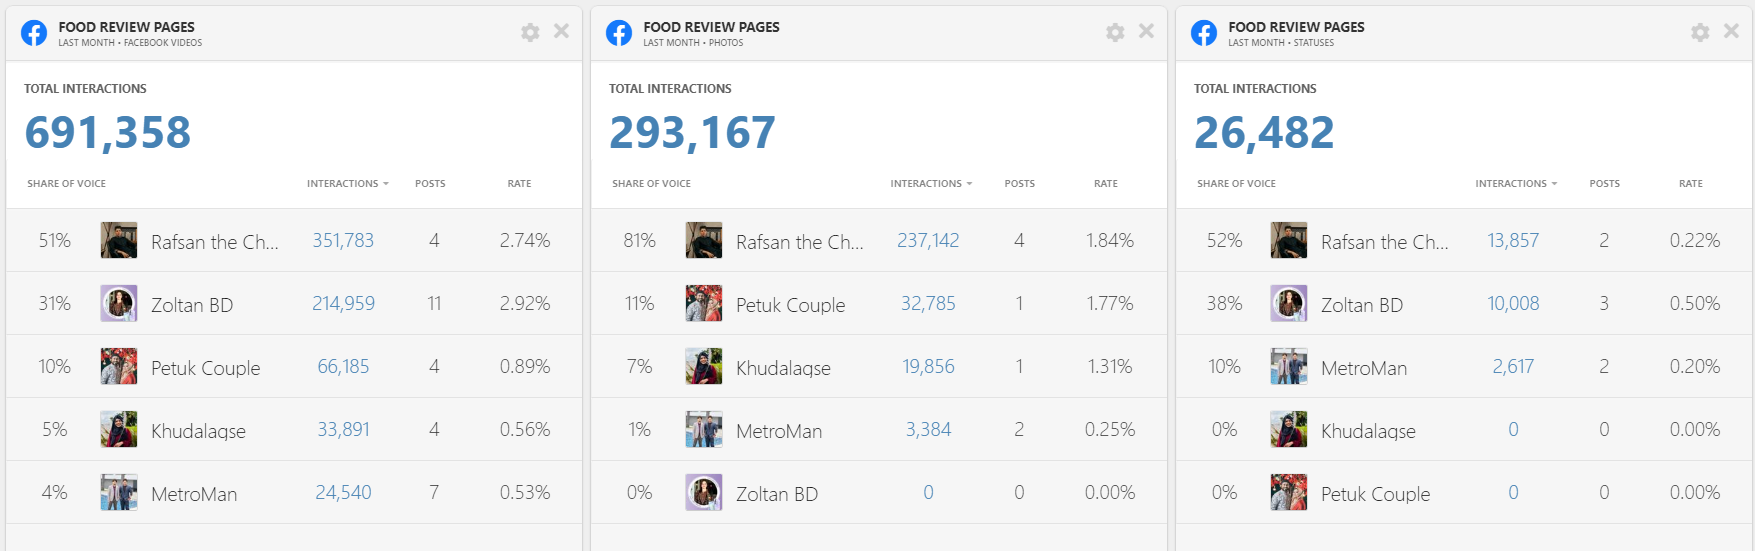
\includegraphics[width=\linewidth]{figures/interaction_content_types.png}
    \caption{Difference between different content types}
    \label{fig_interaction}
\end{figure}

\section{Interaction Data}
We used CrowdTangle \footnote{Website: https://crowdtangle.com/}, a social media analytics tool from Meta. Using CrowdTangle, we selected the top food vloggers and influencers' pages from the dashboard. During this research, we only used the videos published between 2020 to 2022. After downloading the data from CrowdTangle, we filtered the data based on a few conditions such as:
\begin{itemize}
    \item {Post type must be video}
    \item {The content must be posted from their Facebook page/profile}
    \item {The downloaded data must be of a food review video}
\end{itemize}

To fulfill the last condition, we had to manually go to each of the links and check whether it was a food review video or not. If it was not one, we simply discarded the data related to it. Some of the notable data collected from CrowdTangle contained the following information:

\begin{table}
    \begin{center}
        \begin{tabular}{|l|l|}
        \hline
            Post Created Date   & Post Created Time     \\ \hline
            Post Type           & Total Interactions    \\ \hline
            Total Comments      & Shares                \\ \hline
            Likes               & Love                  \\ \hline
            Wow                 & Haha                  \\ \hline
            Sad                 & Angry                 \\ \hline
            Care                & Haha                  \\ \hline
            Sad                 & Total Views           \\ \hline
            Video Length        & Message               \\ \hline
            Link                & Score                 \\ \hline
        \end{tabular}
        \caption{Available Information from CrowdTangle}
        \label{table_crowdtangle_data}
    \end{center}
\end{table}


\section{Comment Data}

Since the Natural Language Processing based approach requires Bangla text to analyze the sentiments of the food review videos, we had to download the comments related to the videos mentioned in the previous section. For the filtered data from the previous section, we had to manually download the comments for each post since no public API exists for Facebook. At the beginning of this study, we had to go to the videos' URL and manually copy-paste the comments to a CSV file. However, as our research progressed, we developed a custom plugin for a Chromium-based browser based on an existing one. The plugin helped us to extract the comments from Facebook easily. For each of the videos, we extracted and saved the comments in an individual CSV file and linked the file to the CSV previously downloaded from CrowdTangle. We took caution while performing this operation since a simple mistake may introduce errors to our findings.

Following the steps above, we downloaded around 26,004 comments from 905 Facebook food review-related videos.


